\def\year{2018}\relax
%File: formatting-instruction.tex
\documentclass[letterpaper]{article} %DO NOT CHANGE THIS
\usepackage{aaai18}  %Required
\usepackage{times}  %Required
\usepackage{helvet}  %Required
\usepackage{courier}  %Required
\usepackage{url}  %Required
\usepackage{graphicx}  %Required

\usepackage[vlined,boxed,ruled]{algorithm2e}
\usepackage{graphicx}
\graphicspath{{figures/}}
\usepackage{subfigure}
\usepackage{amsmath}

\frenchspacing  %Required
\setlength{\pdfpagewidth}{8.5in}  %Required
\setlength{\pdfpageheight}{11in}  %Required
%PDF Info Is Required:
  \pdfinfo{
/Title (2018 Formatting Instructions for Authors Using LaTeX)
/Author (AAAI Press Staff)}
\setcounter{secnumdepth}{0}
 \begin{document}
% The file aaai.sty is the style file for AAAI Press
% proceedings, working notes, and technical reports.
%
\title{2018 Formatting Instructions \\for Authors Using \LaTeX{}}
\author{AAAI Press\\
Association for the Advancement of Artificial Intelligence\\
2275 East Bayshore Road, Suite 160\\
Palo Alto, California 94303\\
}
\maketitle

\begin{abstract}
AAAI creates proceedings, working notes, and technical reports directly from electronic source furnished by the authors. To ensure that all papers in the publication have a uniform appearance, authors must adhere to the following instructions.
\end{abstract}


\section{Introduction}

Associative memory is a new memory storage method. 
The other name content-addressable memory is more clearly. 
It is a special type of computer memory used in certain very-high-speed searching application\cite{krikelis1994associative}.  
The main difference is that a content-addressable memory doesn't need the explicit address which is necessary for traditional computer memory system. 
The associative memory has two types. One is auto-associative memory, and another is hetero-associative. 
In auto-associative memory, the dimension of input is the same with the output. 
In hetero-associative memory, the dimension of input is not the same as the output.

This paper concerns mainly on Hopfield network, one of the auto-associative memory, proposed by John Hopfield in 1982 \cite{hopfield1982neural}. 
He shows that this  network has a complex collective computational  abilities by an ensemble of simple processing units. 
Given an input, the Hopfield model computes its output recursively in time until the system donot change the vector. 
But the  method to design the parameter weight of Hopfield model of which the Hopfield network can remember some memory messages is a big problem. 
In his 1982's original paper, Hopfield designs the prescription of weight which idea is motivated by Hebbian learning rule to achieve the goal, which the Hopfield network can remember some messages, and can recover from the noise messages. 
In 1987, Mceliece proved that the capacity of Hopfield network in his original paper is about 0.14$N$($N$ is the size of the Hopfield network)\cite{mceliece1987capacity}.

Hopfield network is an associative memory network. 
Associative memory is a different memory from traditional memory. 
Traditional memory saves messages at a unique address. When retrieving these messages, we require the complete unique address.
But associative memory can retrieve target message upon only partial information of target message or small error from target message. 
For example, the initial input message is "You are the $\_\_\_$ in my eye." or "You are the appple in my eye.", the target message is "You are the apple in my eye."
This is the capability of an associative network to recall the whole message by the part of message.
So in theorem, Hopfield network can finish this work. 
But there exist some problems, like capacity and recuperative capability.

In my review the Hopfield network, there are two main methods to confirm the weight of the Hopfield network. 
One is designing method, like the Hopfield original paper. 
For instance, In 1987, I. Kanter claim that their method can achieve a better result compared to Hopfield method \cite{kanter1987associative}. 
Then in 1997. Storkey proposed a new designed method to promote the capacity of Hopfield network\cite{storkey1999basins}.  
On the other hand, in 2012, C.Hillaer introduces the minimum probability flow(MPF) to design the weight of Hopfield network by training \cite{hillar2012efficient}. 
However, existing methods to train Hopfield networks  suffer from limited pattern capacity. 
Our method is similar to the MPF, but we can get a better result on all the metric.

Our main theoretical result is that if the Hopfield network has an optimal solution, we can find this optimal solution by machine learning method. 
Besides, if we train on high noise level $\beta$, we can get a better result on noise level under $\beta$. 
We also perform two experiments to verify our theoretical results.

%Our idea is inspired by the prosperous of machine learning method, especially deep neural networks. Deep neural networks achieve many amazing works on image recognition \cite{krizhevsky2012imagenet}, \cite{he2016deep}, large vocabulary speech recognition

In the remainder of the paper, we discuss the previous work on weight setting of the Hopfield network. 
Then, we give the notation and terminology. 
Next, we perform theorem results and prove them. Then we present our algorithm to solve problems. 
In the experiment part, we first introduce our simulation dataset. 
Next we give the comparison of method. Then we give our two experiment result. 
Finally, we summarise our work and give the direction of future work. 

\section{Discussion of Previous Work}

Hopfield network is a $N$ nodes of a network. 
This is a system with $N$ dimension state. The parameter of the system is $\textbf{W}$. 
If you input a probe of $N$ dimension vector, the system will output the target message of the probe after the evolution. 
The critical problem is how to get the parameter weight $\textbf{W}$ of which the system can remember some messages and do recovery work.

There are two research directions to get the parameter weight $\textbf{W}$ of the system. 
On one hand, set weight by memory messages, particularly like Hopfield's work in 1982\cite{hopfield1982neural}, Pseudo-inverse learning rule by I. Kanter in 1987\cite{kanter1987associative}, and Storkey learning rule by A. Storkey in 1999\cite{storkey1999basins}. 
On the other hand, there is a machine learning method introduced by C. Hillar in 2012\cite{hillar2012efficient}. 
Our method is also machine learning method, but different from MPF in exact learning method, and we can get better results.

\subsection{Hopfield Method}
A learning rule can have two useful properties: local and incremental. 
If it uses only the information from both nodes whose connectivity weight is updated for each update, we call it local. 
If it does not require any information about the other patterns previously learnt by the network, we call it incremental.

$X_i^m$ is the state of node $i$ in message $m$. $W_{ij}^m$: the weight after $m^{th}$ memory message saved.

Hopfield designed the weight of this system by Hebbian learning rule. 
He presented the associative memory function by experiment. 
And he gave a simple explain which the capacity of Hopfield network is $0.14N$. 
Hopfield network is local and incremental.
The main learning method is according to the following equation:
    \begin{eqnarray*}
     W_{ij}^0 = 0 \quad and \quad W_{ij}^m = W_{ij}^{m - 1} + \frac{1}{N} X_i^mX_j^m
    \end{eqnarray*}

Then in 1987, I.Kanter proposed a learning rule named pseudo-inverse which the capacity is $N$. But this method is neither local nor incremental.
    \begin{eqnarray*}
     W_{ij} = \frac{1}{N} \sum_{v=1}^M \sum_{\mu = 1}^M X_i^v(Q^{-1})^{v\mu}X_j^{\mu}
    \end{eqnarray*}

Then in order to get a larger capacity, A.Storkey proposed a new learning rule in 1997 which is not only local but incremental.
    \begin{eqnarray*}
     W_{ij}^0 &=& 0; \\
     W_{ij}^m &=& W_{ij}^{m - 1} + X_i^mX_j^m - X_i^mh_{ji}^m - h_{ij}^mX_j^m \\
     h_{ij}^m &=& \sum_{k=1,k\neq i,j}^N W_{ik}^{m-1}X_k^m
    \end{eqnarray*}

\subsection{MPF}
C.Hillar introduced minimum probability flow(MPF) which is a parameter optimization method in energy-based probabilistic models. 
He insisted that his algorithm achieves $N$ storage which is at least one pattern per neuron. 
The weight from his method can also get a better recovery ability on noisy or corrupted versions of a stable point of pattern.

Consider a collection of $M$ N-bit messages $\cal{D}$ to be stored as strict local minima in a Hopfield network. $\cal{N}(X)$: The neighborhood of $X$ consists of those vectors which are Hamming distance 1 away from $X$. 
The minimum probability flow(MPF) objective function given the collection $\cal{D}$ is
    \begin{eqnarray*}
      K_{\cal{D}}(W, \theta) := \sum_{X \in \cal{D}} \sum_{X' \in \cal{N}(X)} \exp \left(\frac{E_x - E_{x'}}{2}\right)
    \end{eqnarray*}
Notice that this function is infinitely differentiable and convex in the parameters.
Minimizing this objective function given a storable set of patterns will determine a Hopfield network storing those patterns.

\subsection{Our method}
Since there is a solution of weight $\textbf{W}$ which can save memory messages. 
So in theory, there is an optimization method we can find this solution or an approximate solution. 
So according to the structure of Hopfield network, we design this MLP network to simulate the Hopfield network. 
After training on the training set, the approximate solution we can obtain. 
The main contribution of our work is:
\begin{itemize}
  \item Our machine learning method can get the approximate solution of the Hopfield network.
  \item Prove that if we train the Hopfield network on noise level $\beta$, the message error is less than $\epsilon, \forall \epsilon$. 
      then $\forall \gamma < \beta$, the $\gamma$ is noise level on the testing set, the message error is also less than $\epsilon$.
      And this conclusion can be verified by the experiment.
  \item The simulation experiments also exhibit that the weight $W$ of our MLP method can get a better result in recovery problem.
\end{itemize}

\section{Definitions and Terminology}
\subsection{Definitions}


In Hopfield original paper, the Hopfield network $\cal{H} = (\textbf{W}, \theta)$ with $N$ nodes. 
So the state is $N$-dimension vector, the weight matrix $\textbf{W}$ is symmetric with zero diagonal, and the $\theta = (\theta_1,...,\theta_N)^T$ is a threshold vector. 
The state $X$ choose from binary vector $\{0, 1\}^N$, represented by $X = (x_1, ..., x_N)^T$. 
Given any probe $X$ to the Hopfield network, there will be a dynamical update of $X$ in every position $x_i$ according to
\begin{eqnarray*}
% \nonumber % Remove numbering (before each equation)
  x_i &=& H(\textbf{W}_iX - \theta_i)
\end{eqnarray*}
Here, $\textbf{W}_i$ is the $i$-th row of $\textbf{W}$ and $H$ is the Heaviside function of which

\begin{eqnarray*}
  H(r) = 
  \begin{cases}
    1, & \mbox{if $r > 0$} \\
    0, & \mbox{otherwise}.
  \end{cases}
\end{eqnarray*}
In summary, the every position of unit compute a weighted sum of the input and produces binary result depending on whether the weighted sum is below or above a certain threshold value.

The energy of Hopfield network with a binary pattern $X$ is defined by
\begin{eqnarray*}
% \nonumber % Remove numbering (before each equation)
  E_X(\textbf{W}, \theta) &:=& -\frac{1}{2}X^T\textbf{W}X + \theta^TX \\
  &=& -\frac{1}{2}\sum_{i=1}^{N} \sum_{j=1}^{N} W_{ij}x_ix_j + \sum_{i=1}^{N} \theta_ix_i
\end{eqnarray*}
This is identical to the energy function for an Ising model in physics. 
Besides, Hopfield proves that under asynchronous dynamical updates, the energy cannot increase. 
Thus, after a finite updates, the probe will converge to a stable point $X^*$, of which $x_i^* = H(\textbf{W}_iX^* - \theta_i)$ for each $i$.

Given $\mathcal{M} = \{X^1, ..., X^M\}$, where each $X^i$ is an i.i.d. \emph{Ber}($\alpha$) sequence. For each $X^m$, let$Y^{mk} = \bar{X}^m$, every position $y_i^{mk} = \bar{x}_i^m$ with a probabilistic $\beta$. Otherwise, $y_i^{mk} = x_i^m$. The objective function is:
\begin{eqnarray*}
% \nonumber % Remove numbering (before each equation)
  F(\textbf{W}, \theta) &:=& \sum_{m=1}^{M}  \textbf{E}_{Y^{mk}} ||g_1(Y^{mk}, \textbf{W}, \theta) - X^m||^2
\end{eqnarray*}

If $X$ is binary vector, $g_1$ is sigmoid function with parameter $\sigma$. 
When $\sigma \rightarrow \infty$, we know sigmoid function is the Heaviside function. 
This is why we choose this continue function to approximate the Heaviside function. Cause sigmoid function is a continue function, we can do partial derivative on weight $\textbf{W}$.

\subsection{Theorem Results}
Theorem I: If we train the Hopfield network on noise level $\beta$, the error rate is $\epsilon_1$. 
Then we conclude that if the testing set's noise level is low than $\beta$, the error rate is low than $\epsilon_1$.

Cause this is an evolution system, every state vector will arrive a state. 
After our training, we get a weight $\textbf{W}$ to make messages $\mathcal{M}$ stable point with an attraction domain. 
Then for any probe input $X$, there are three cases:
\begin{itemize}
  \item $X$ is in true attraction domain, then the output is the true memory.
  \item $X$ is in false attraction domain, then the output is the false memory.
  \item $X$ is not in attraction domain, then the output is false.
\end{itemize}

For every $X^m$, there is a radius $D^m$ of attraction domain. 
If we choose $Y^{mk}$ from the $Ber(\beta)$. 
The probabilistic is $Er = \frac{1}{M} \sum_{m=1}^{M}Er(D^m)$, where $Er(D^m) = 1 - \sum_{d=1}^{D^m} C_N^d \beta^d (1 - \beta)^{N-d}$. 
According the distribution of $Ber(\beta)$, the following conclusion is correct.
Along with the increase of $\beta$, the error rate is increased.

On the other hand, we can get the exact error function with the parameter $\beta$.
Let fix $x_i$, the random is come from $Y$ and $x_k, k \neq i$. Mark $h_i = W_{ii}Y_i + \sum_{k \neq i}^N W_{ik}Y_k$. When $X_i = 1$, $$E(h_i|X_i = 1) = W_{ii}(1 - \beta) + \sum_{k \neq i}W_{ik} [\beta \bar{X_k} + (1 - \beta) X_k]$$
Moreover, $$E(h_i|X_i = 1) = W_{ii}(1 - \beta) + \sum_{k \neq i}W_{ik} [\beta (1 - \alpha) + (1 - \beta) \alpha]$$
Let $R_k = W_{ik}[\beta \bar{X_k} + (1 - \beta)X_k]$, we know $R_k$ is a independent random variables, each with finite expected value $\mu_k$ and variance $\sigma_k^2$.
\begin{eqnarray*}
  \mu_k &=& W_{ik}[\beta (1 - \alpha) + (1 - \beta) \alpha] \\
  \sigma_k^2 &=& W_{ik}^2 [\beta^2 + (1 - \beta)^2](1 - \alpha)\alpha
\end{eqnarray*}
According to the Lyapunov Central Limit Theorem, when $N \rightarrow \infty$, we know $\sum_{k \neq i}^N R_{k}$ is a Gaussian distribution with $$\mu = \sum_{k \neq i}^N W_{ik}[\beta (1 - \alpha) + (1 - \beta) \alpha]$$
and $$\sigma^2 = \sum_{k \neq i}^N W_{ik}^2 [\beta^2 + (1 - \beta)^2](1 - \alpha)\alpha$$

Then we get the results: When $X_i = 1$, and $N$ is a big number, $h_i$ is a Gaussian distribution.
    \begin{eqnarray*}
      \mu_{h_i^1} = W_{ii}(1 - \beta) + \sum_{k \neq i}^N W_{ik}[\beta (1 - \alpha) + (1 - \beta) \alpha] \\
      \sigma_{h_i^1}^2 = \sum_{k \neq i}^N W_{ik}^2 [\beta^2 + (1 - \beta)^2](1 - \alpha)\alpha
    \end{eqnarray*}
When $X_i = 0$, and $N$ is a big number, $h_i$ is a Gaussian distribution.
    \begin{eqnarray*}
      \mu_{h_i^0} = W_{ii} \beta + \sum_{k \neq i}^N W_{ik}[\beta (1 - \alpha) + (1 - \beta) \alpha] \\
      \sigma_{h_i^0}^2 = \sum_{k \neq i}^N W_{ik}^2 [\beta^2 + (1 - \beta)^2](1 - \alpha)\alpha
    \end{eqnarray*}
Notice that the $\mu_{h_i^1}$ is different from $\mu_{h_i^0}$, the $\sigma_{h_i^1}$ is the same with $\sigma_{h_i^1}$, we abbreviate it as $\sigma_{h_i}$. 
So bit error rate(\textbf{BER}) and message error are as follows:
    \begin{eqnarray*}
      \textbf{BER}_i &=& \phi(\mu_{h_i^1}, \sigma_{h_i};\frac{1}{2}) + [1 - \phi(\mu_{h_i^0}, \sigma_{h_i}; \frac{1}{2})] \\
      \textbf{BER}_{max} &=& \max_{i} \textbf{BER}_i \\
      \textbf{MER} &=& 1 - (1 - \textbf{BER}_{max})^N
    \end{eqnarray*}
Since $\textbf{BER}_{max} \in [0, 1]$, $\textbf{MER}$ is increased with $\textbf{BER}$. 
Cause $\textbf{W}$ is not all positive, so we cannot get the relation of $\textbf{BER}_{max}$ and $\beta$, or $\textbf{MER}_{max}$ and $\beta$.

\subsection{Algorithm}

 According to the purpose of remembering messages, we generate the training set from the memory messages. 
 Then we design the objective function to achieve our goal. 
 Exactly, we metric the Euclid distance between the output of Hopfield system and the label.
 
 This is a optimization problem. So we adopt stochastic gradient descent(\textbf{SGD}) algorithm to train $F(\textbf{W})$, then we get the optimal $\textbf{W}$, and mark it as $\textbf{W}^*$, note that $\textbf{W}^*$ depends on $\{ \mathcal{M}, \beta, N\}$.

 The exact algorithm is as follows:

\begin{algorithm}[tbp]
\LinesNumbered
\caption{MLP Training}\label{MLP Training}
\KwIn{$E, \{X^i, Y^i\}_{i=1}^{A}$}
\KwOut{$\textbf{W}$}
Initialization:
$\textbf{W}$\;
\While{$e<E$}{
    Sample a minibach $\{(X^i, Y^i)\}, i = 1, ..., B$\;
    \For {$i = 1, ..., B$}{
        Computer the gradient:
        $\Delta \textbf{W} \leftarrow \nabla_{\textbf{W}}l(\textbf{W}, \{(X^i, Y^i)\})$\;
        $\textbf{SW} \leftarrow \textbf{SW} + \Delta \textbf{W}$\;
        }
    $\textbf{W} \leftarrow \textbf{W} - \epsilon \cdot \textbf{SW}$\;
    \For {$i = 1, ..., A$}{
        Calculate the loss $l_i$:
    }
    Calculate the loss on Training set:
    $L = \sum_{j=1}^{B} l_j$\;
    \If {$e > 100$}{
        $\Delta L \leftarrow |L(e)-L(100)|$\;
        \If {$\Delta L < \delta$}{
            stop
        }
    }
    $e \leftarrow e + 1$
}
\Return  $\textbf{W}$\;
\end{algorithm} 

\section{Experiment}

We evaluate the effectiveness of our MLP method with the Hopfield original network on MER(Message error) and BER(Bit error). We also do many experiments on different weight setting method of Hopfield network on different noise level. We do the experiments like Hopfield's original paper. The details of the datasets, the models and the training routines are summarized below.

\subsection{Datasets}

Our experiments are simulation. So the datasets are generated random. In our experiments, the Hopfield network's size are 30 and 100. The number of memory messages are 2,4,6 on 30 size, 10,15,20 on 100 size. For instance, we random generate 10 messages on 100 size. Every message is drown from a length of 100 $Ber(1/2)$ sequence. So message is a $100$ dimension binary vector, and every position choose from $\{-1, 1\}$ with probability $1/2$. Then for every position of every memory message, we generate 300 noise vectors by the following rule. For every position of memory message, we reverse its value, i.e 1 to -1, or -1 to 1, with probability of noise level. The noise levels we used are 0.05, 0.1, 0.2, 0.3.

There are two datasets. First, for every noise level, we generate memory messages. Then we generate the training set and testing set on this noise level. Second, on noise level 0.3, we generate memory messages, and generate training set. Then we according to these messages, generate testing set on noise level 0.1, 0.2, 0.3.

After this, we get a size of 3k training sets. Then we use the same method to generate the testing sets of which size is also 3k. In summary, on size 30, for message memory 2, we get 600 dataset. For message memory 4, we get 1.2k dataset. For message memory 6, we get 1.8k dataset. On size 100, for message memory 10, we get 3k dataset. For message memory 15, we get 4.5k dataset. For message memory 20, we get 6k dataset.

\subsection{Models and Implementation details}
\subsubsection{Hopfield method}

There are three Hopfield method. First is the Hopfield original paper. We call it HOP. Its idea of weight setting comes from Hebbian learning. Second is the pseudo-inverse method, called PSE. Third is the Storkey method, called STO. All these methods have a common property which don't need training step. The parameter weight of system is set only by the memory messages. So we just evaluate it on testing set.

\subsubsection{Machine learning method}

There is a new method different from the Hopfield method, called MPF. Its idea comes from minimum probability flow(MPF). It is a method similar to machine learning method. Cause we need to minimise a objective function to get the optimal weight. The difference is the objective function. In our method, we minimise the Euclid distance in training set. But the MPF minimise the energy between the message and its neighborhood. Our method is true from machine learning. We construct the training set according to our goals. So our methods can get better results on this task in theory. And the experiments also exhibit this result.

\subsubsection{Evaluation metric}

There are three metrics to evaluate the efficient between different methods. First, we call it MER, mean message's error. It requires that all the bit of message is the same with the target message. The second metric is BER, which means the bit error. The third metric is the most important metric, we call it Instability. Though the recovery is our objective, the memory messages are stable point.

\subsection{Results}

\subsubsection{Experiment I}

We do these experiments on 100 nodes. The memory messages are 10, 15 and 20. This experiment showed that our method MLP consistently superior to the antecedent weight setting method in all three metrics.

First in 10 memory messages. On noise level 0.05, 0.1, and 0.2, our MLP method is same efficiency with PSE and STO on metric MER, BER and Ins. On noise level 0.3, we can find the superiority of our method. Our MLP method is better than PSE, then STO, then MPF, and the last is HOP on MER and BER. About the Ins, the experiments show that MLP, PSE and STO all stable in all noise level. The worst result is HOP, but 0.04 is on 10 messages. So the wrong message is less than 1. Because we do the same experiment on 50 trial. This result is the mean of all these 50 trails. Maybe in some trials, there are two memory message is similar, so one of them is not stable.

%\begin{figure*}[!h]
%  \begin{minipage}{0.35\linewidth}
%    \centering
%    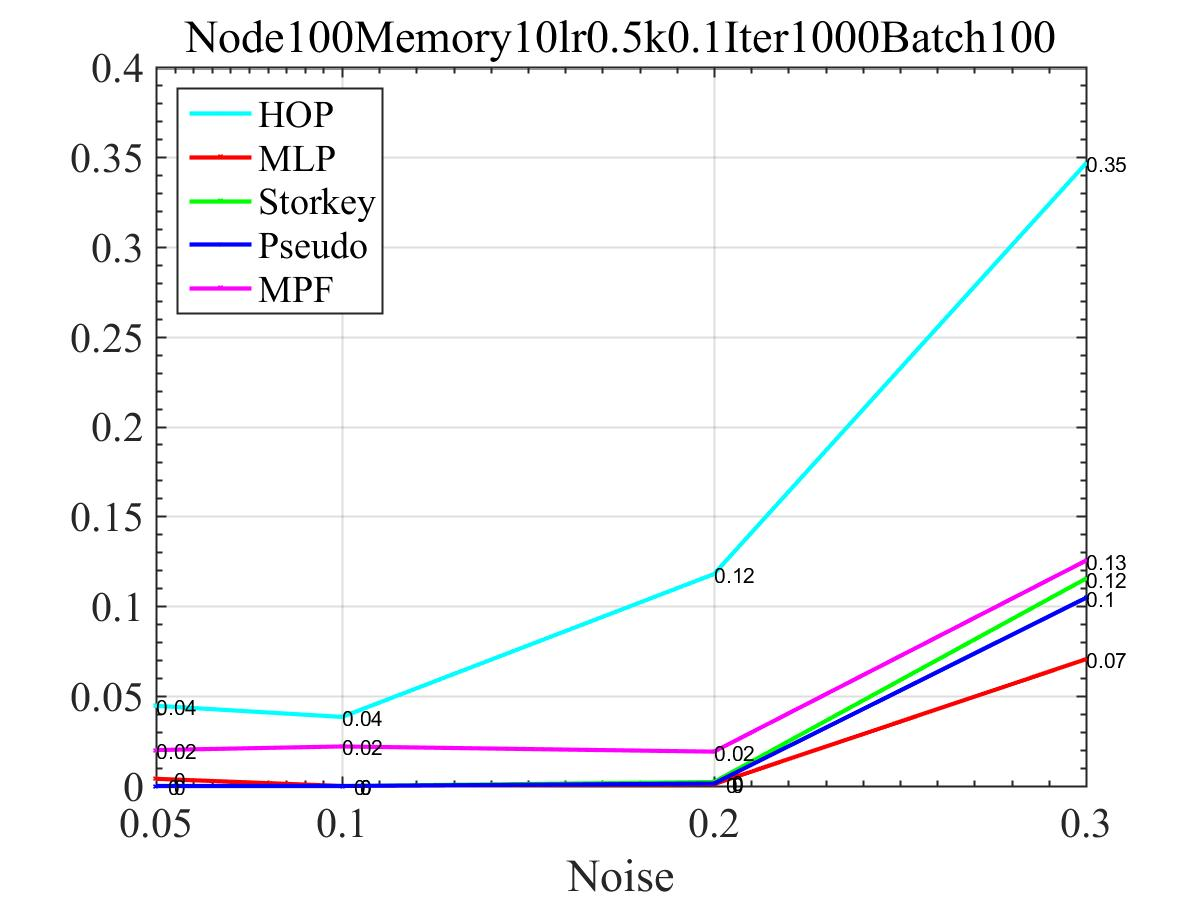
\includegraphics[width=0.8\textwidth]{Memory10MER.jpg}
%    \label{fig:figure1a}
%  \end{minipage}
%  \begin{minipage}{0.35\linewidth}
%    \centering
%    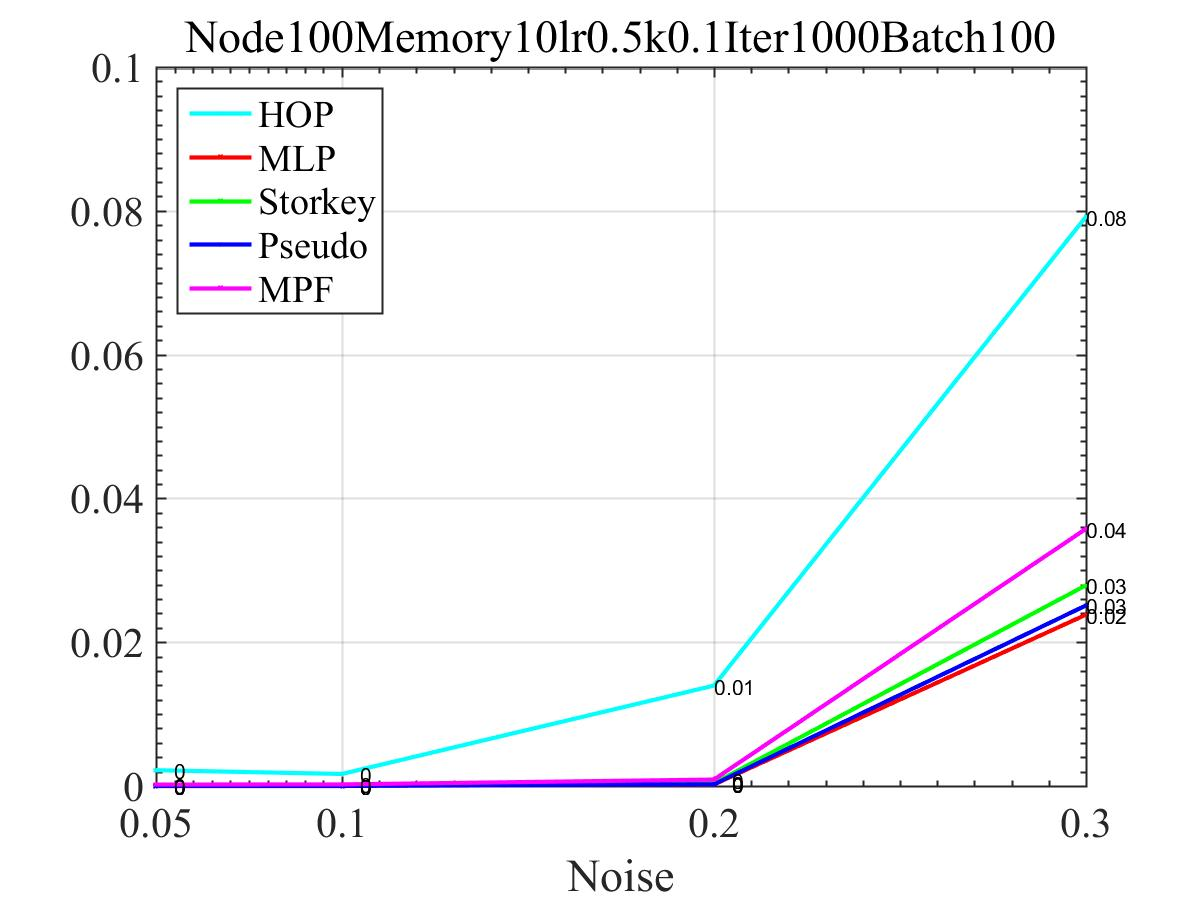
\includegraphics[width=0.8\textwidth]{Memory10BER.jpg}
%    \label{fig:figure1b}
%  \end{minipage}
%  \begin{minipage}{0.35\linewidth}
%    \centering
%    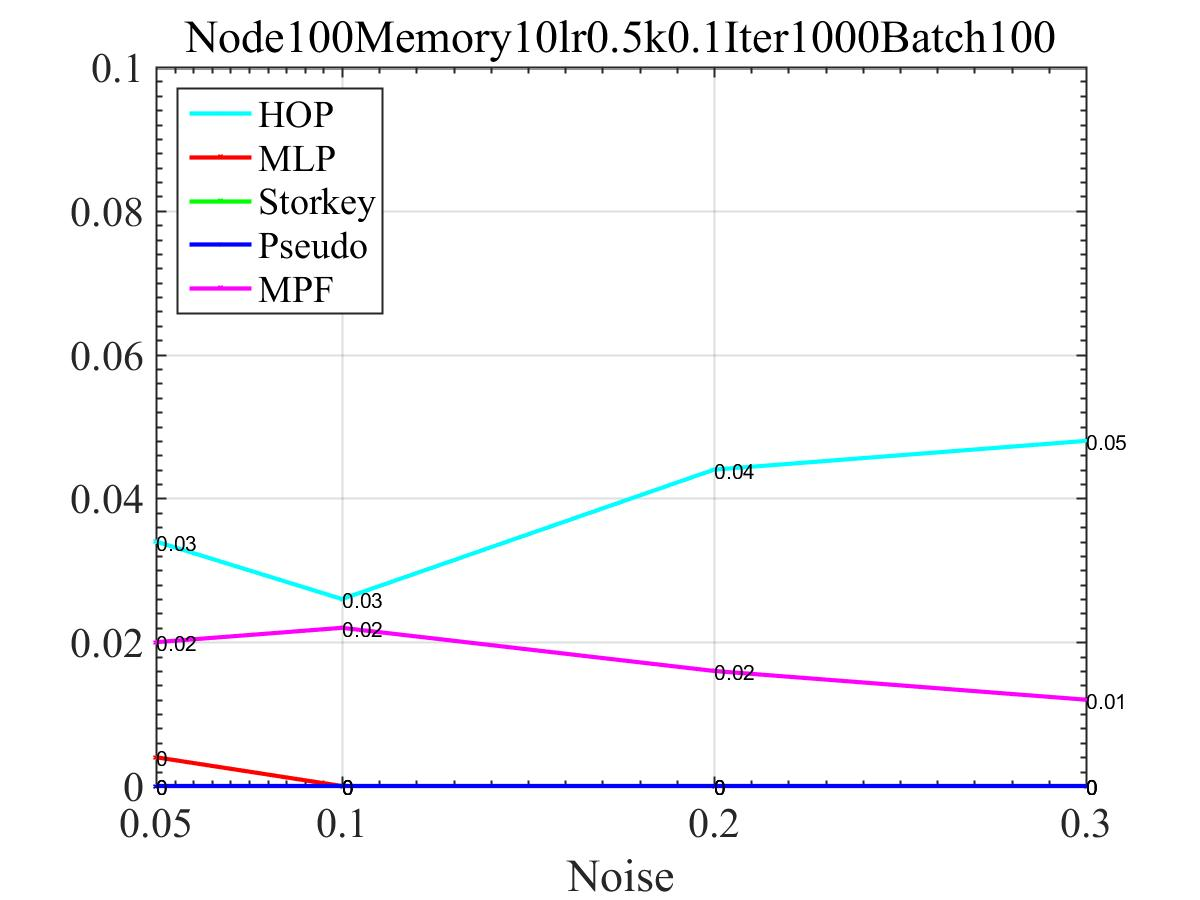
\includegraphics[width=0.8\textwidth]{Memory10Ins.jpg}
%    \label{fig:figure1c}
%  \end{minipage}
%  \caption{Memory10}
%\end{figure*}

\begin{figure*}[!h]
  \subfigure[MER]{
  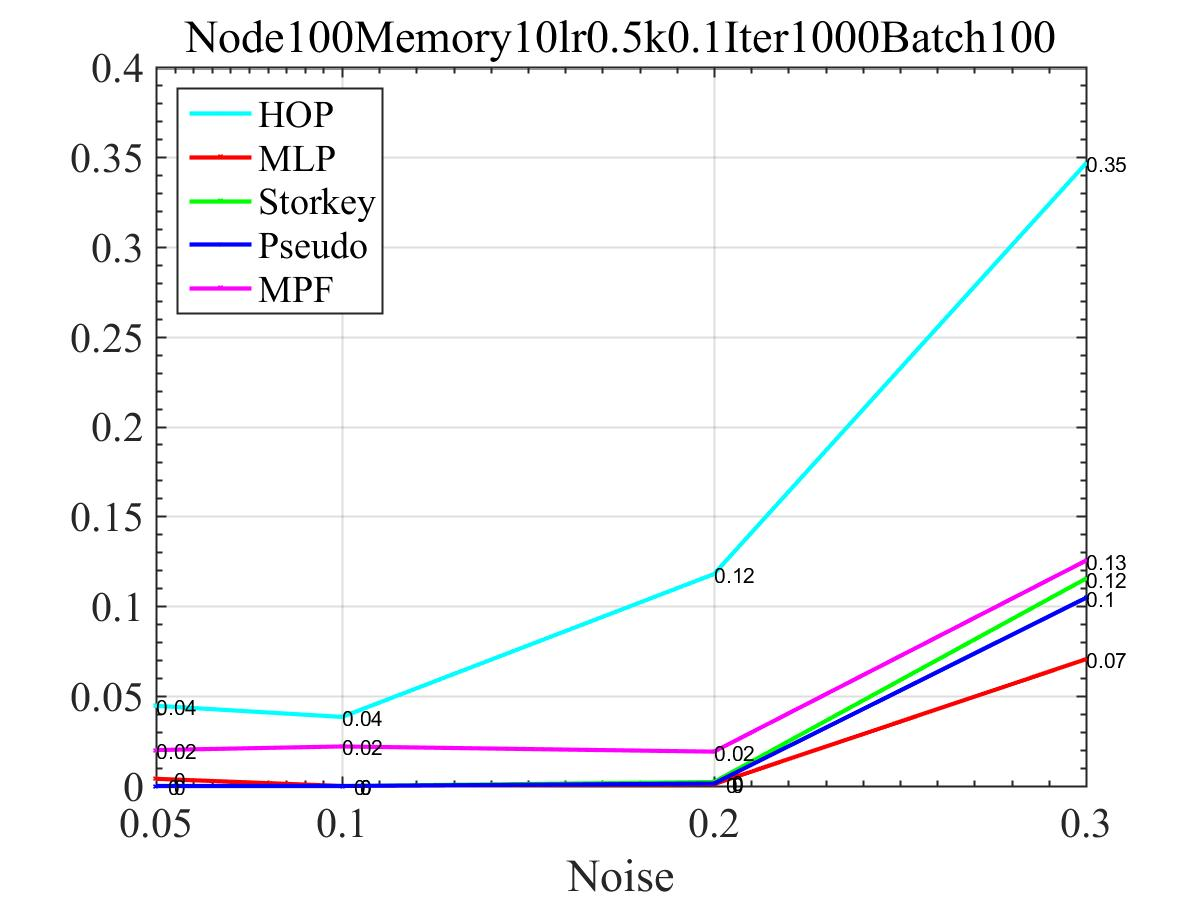
\includegraphics[width=0.35\textwidth]{Memory10MER.jpg}}
  \subfigure[BER]{
  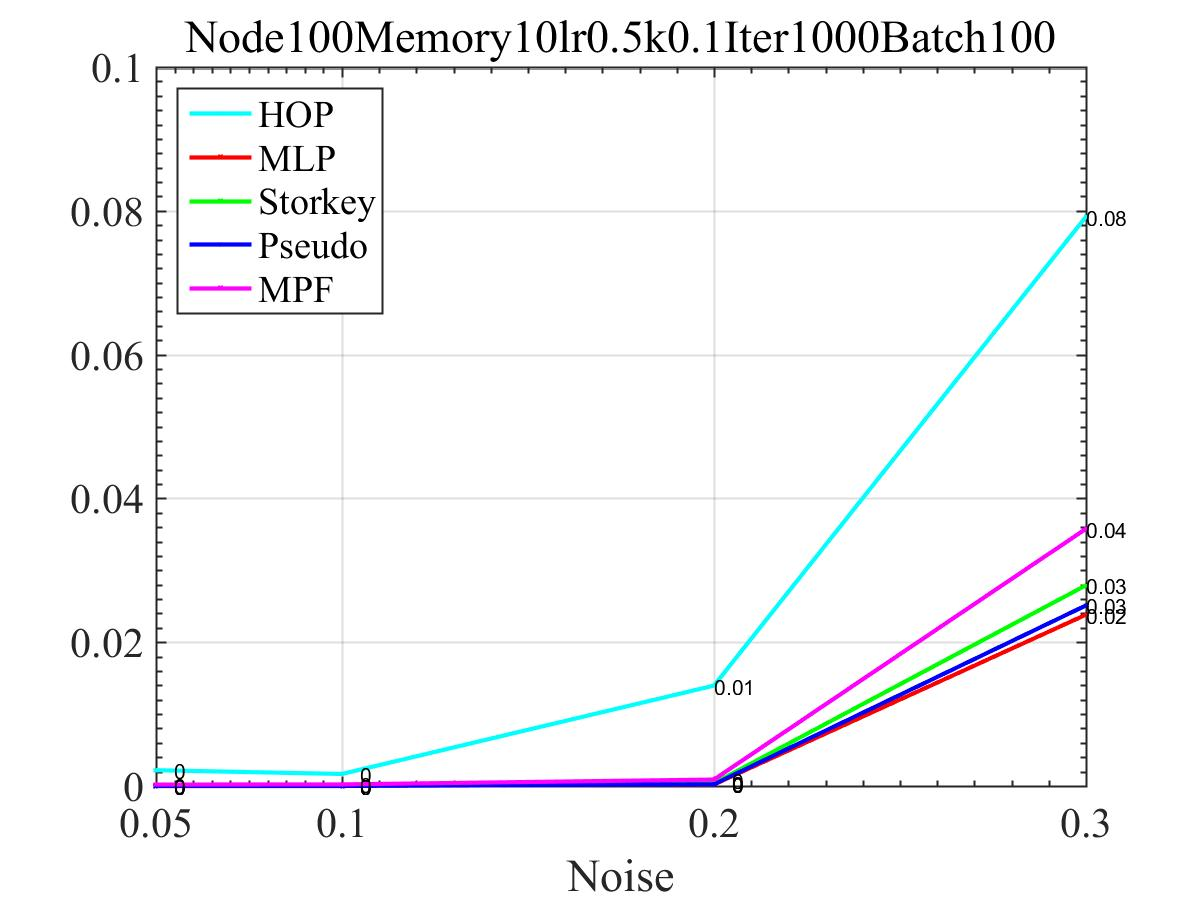
\includegraphics[width=0.35\textwidth]{Memory10BER.jpg}}
  \subfigure[Ins]{
  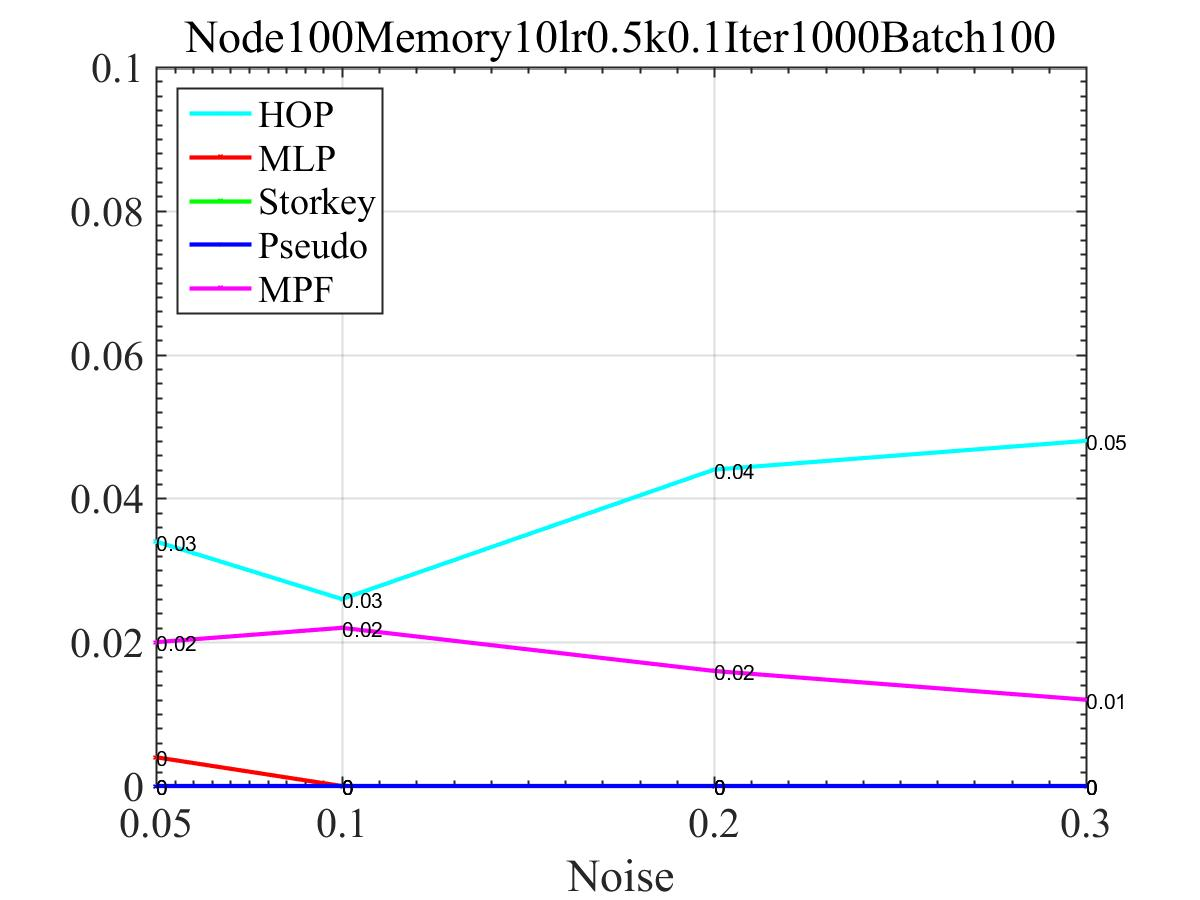
\includegraphics[width=0.35\textwidth]{Memory10Ins.jpg}}
  \caption{Memory10}
  \label{fig:fig1}
\end{figure*}


Second in 15 memory messages. Since the number of memory messages exceeds the capacity of Hopfield original network. In figure \ref{fig:fig2}, in all noise level, the error is about 3 memory messages of 15 memory messages. This accords with the theory of capacity of Hopfield network which the capacity is 0.14$N$. And on noise level 0.05, the MLP method have 0.03 error rate. This causes that MER also have 0.03 error rate.  But MPF, PSE, STO and our method MLP are almost stable on memory messages. So in figure \ref{fig:fig2} and \ref{fig:fig2}, on noise level 0.05, 0.1, and 0.2, the error rate is almost the same in all methods except HOP on metric MER and BER. The advantage of our method MLP is on noise level 0.3, both on metric MER and BER, our method MLP superior to MPF, then PSE, then STO, last is HOP.

\begin{figure*}[!h]
  \subfigure[MER]{
  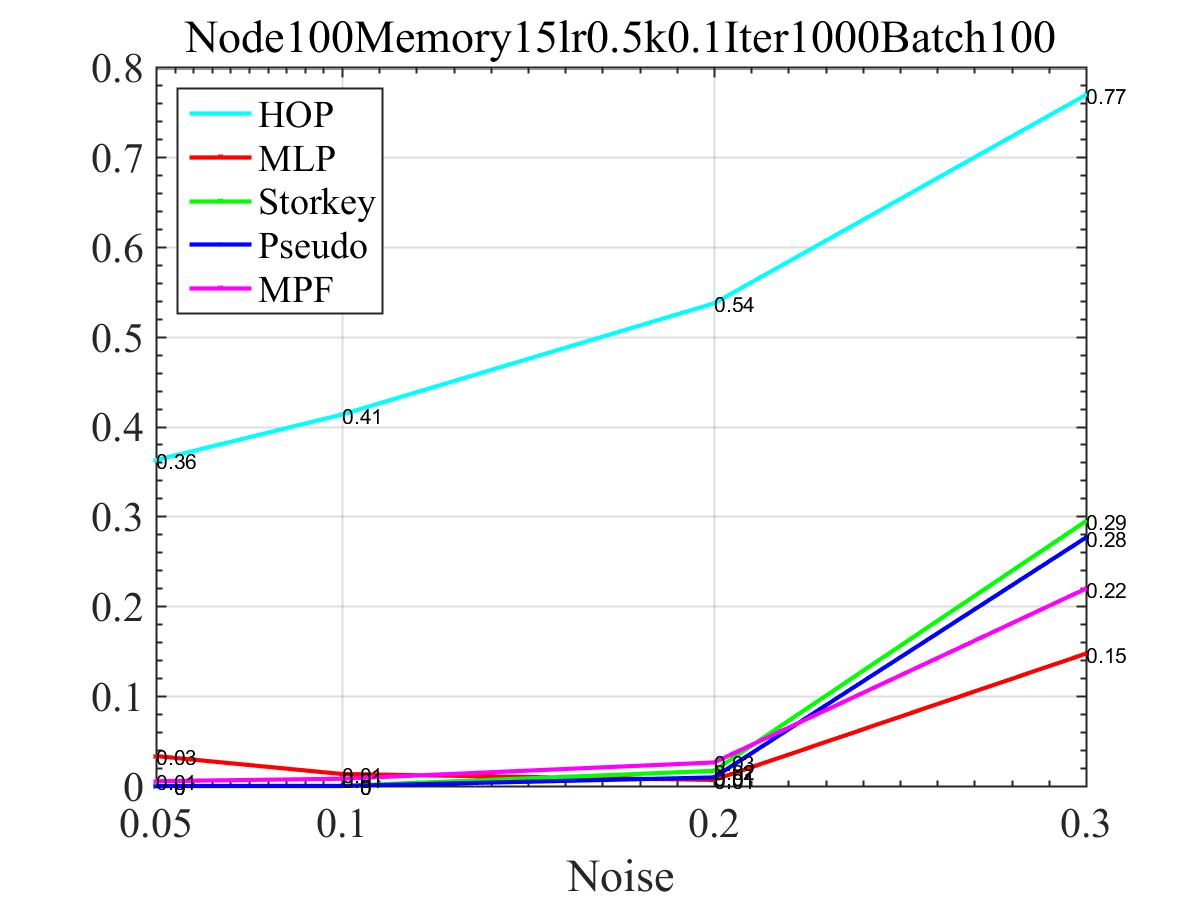
\includegraphics[width=0.35\textwidth]{Memory15MER.jpg}}
  \subfigure[BER]{
  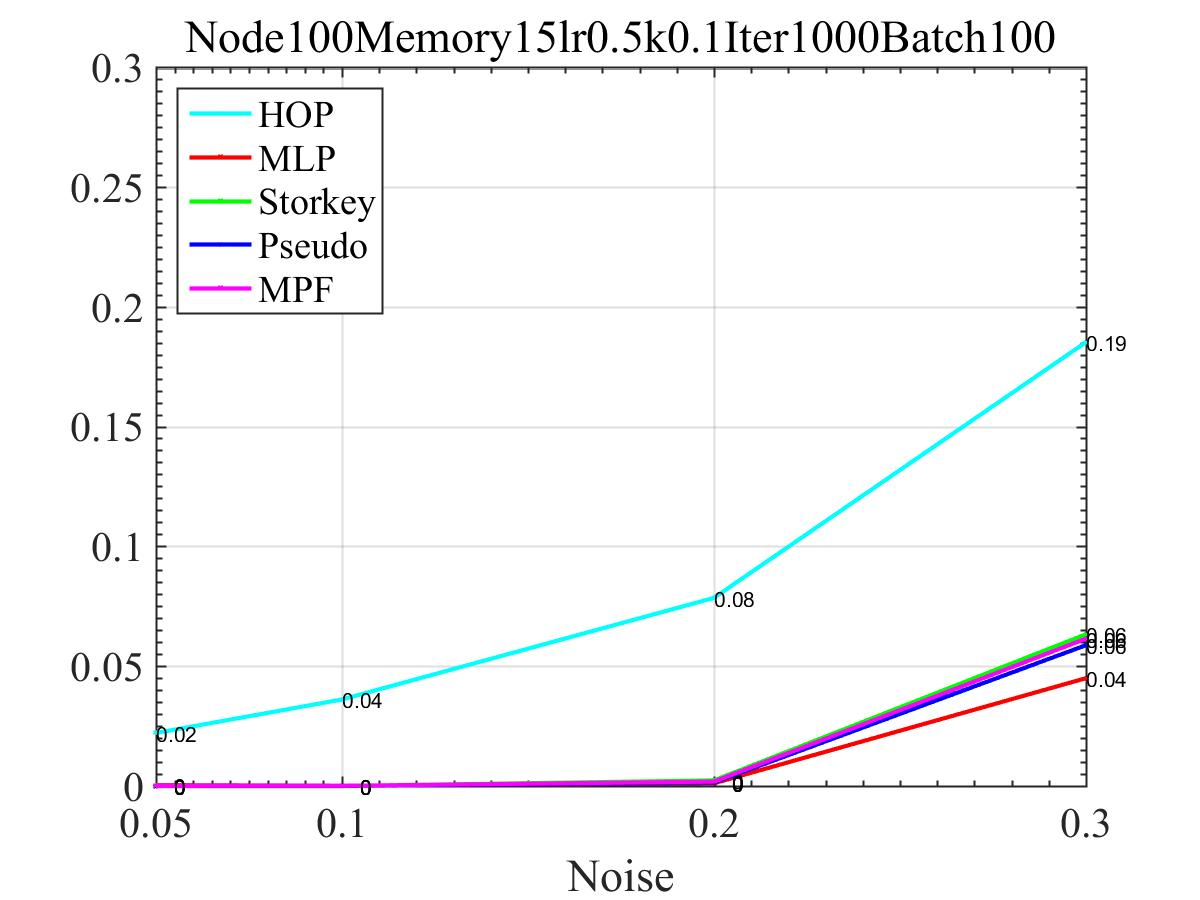
\includegraphics[width=0.35\textwidth]{Memory15BER.jpg}}
  \subfigure[Ins]{
  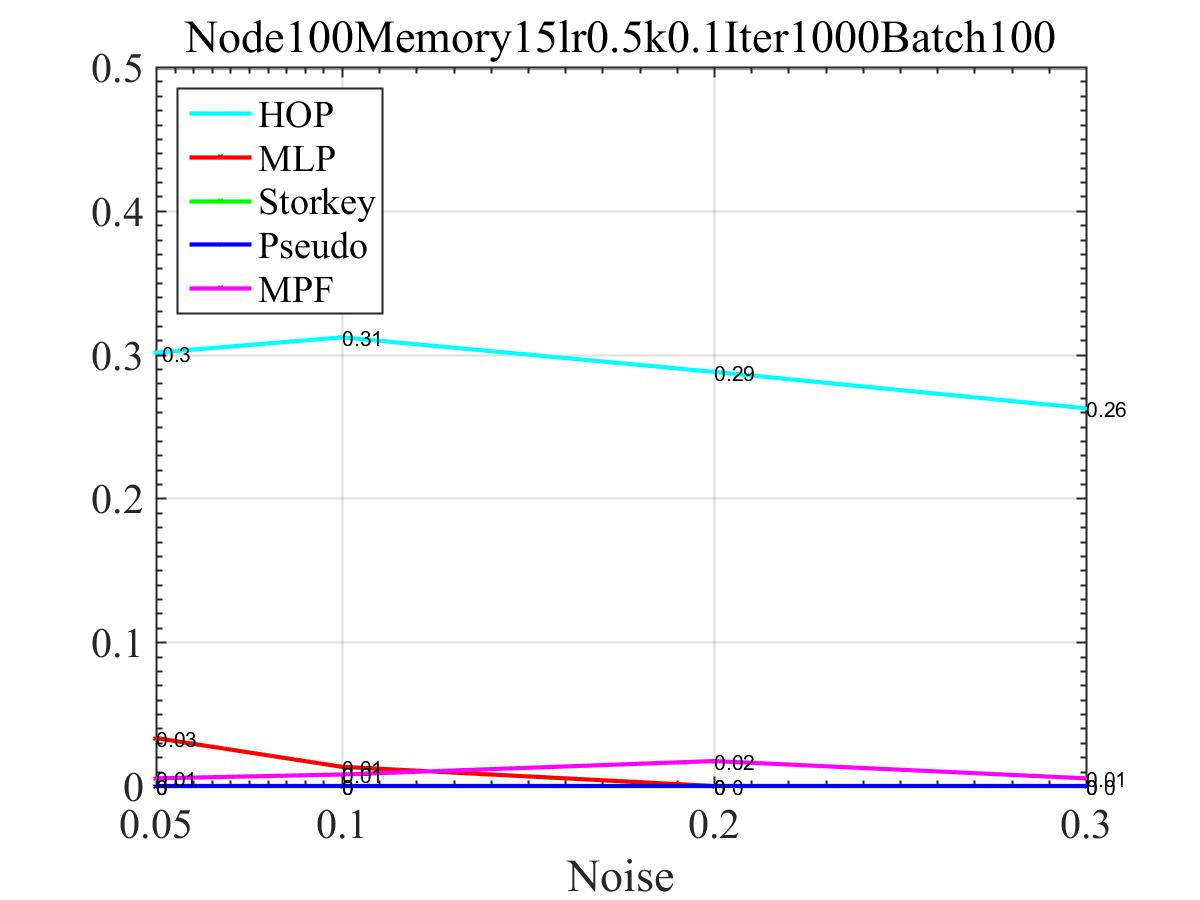
\includegraphics[width=0.35\textwidth]{Memory15Ins.jpg}}
  \caption{Memory15}
  \label{fig:fig2}
\end{figure*}
%
%\begin{figure}
%  \centering
%  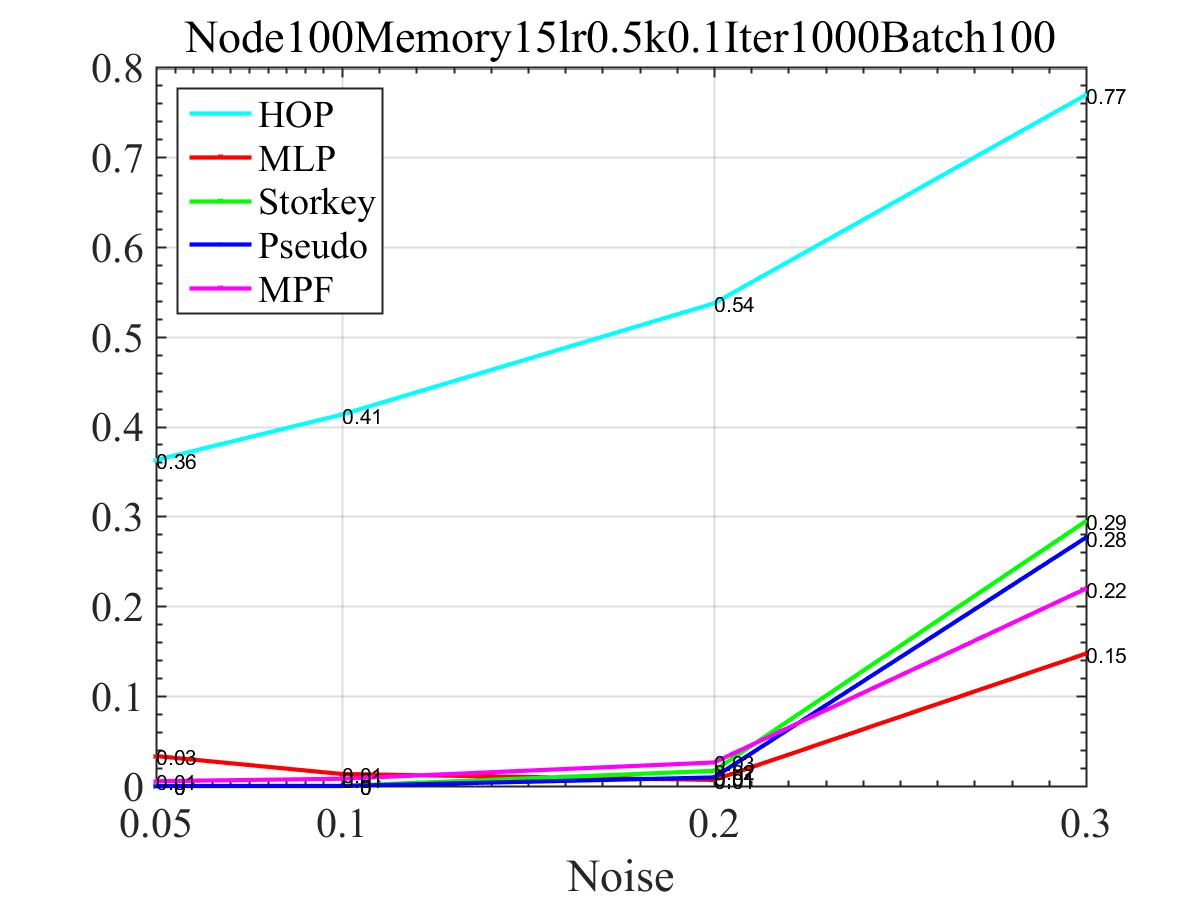
\includegraphics[width=2.2in]{Memory15MER.jpg}
%  \caption{Memory15MER}\label{fig:side:2a}
%\end{figure}
%\begin{figure}
%  \centering
%  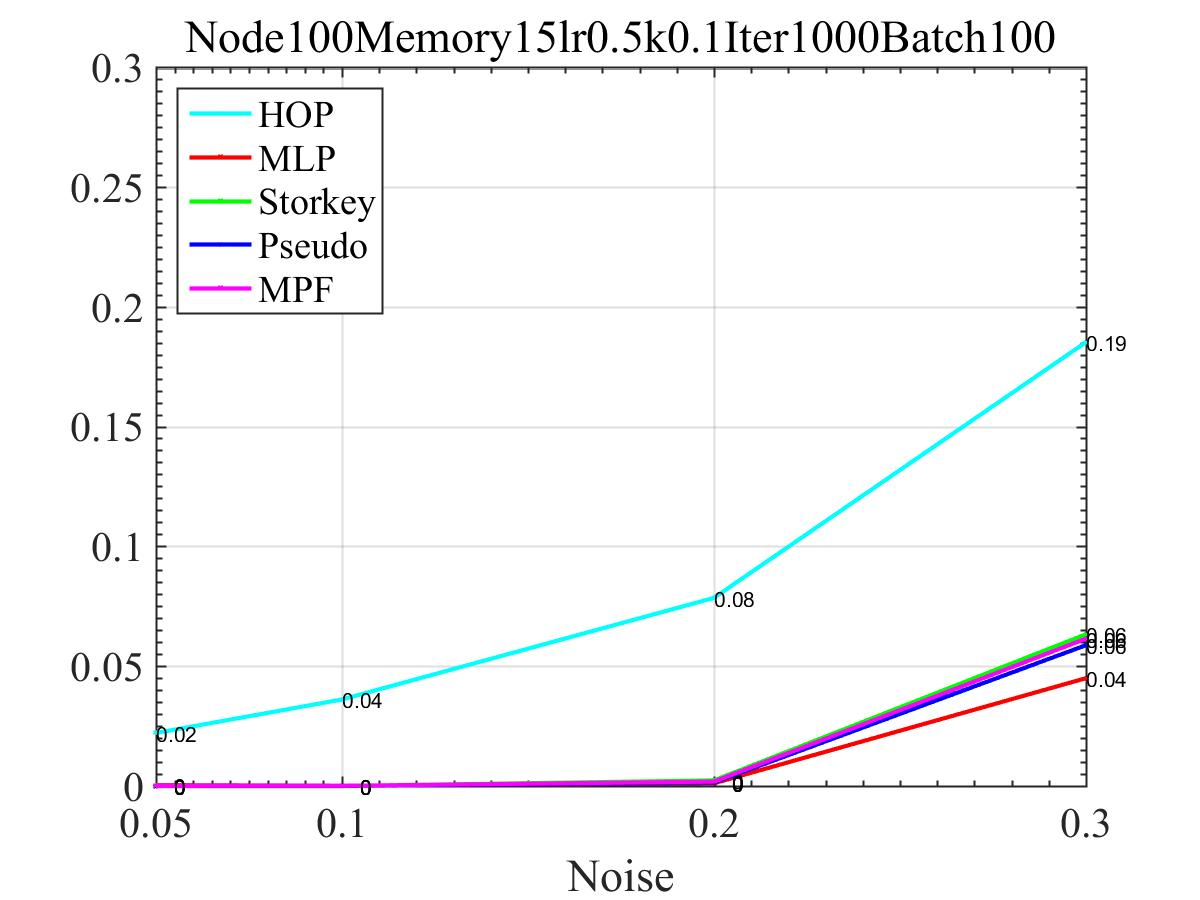
\includegraphics[width=2.2in]{Memory15BER.jpg}
%  \caption{Memory15BER}\label{fig:side:2b}
%\end{figure}
%\begin{figure}
%  \centering
%  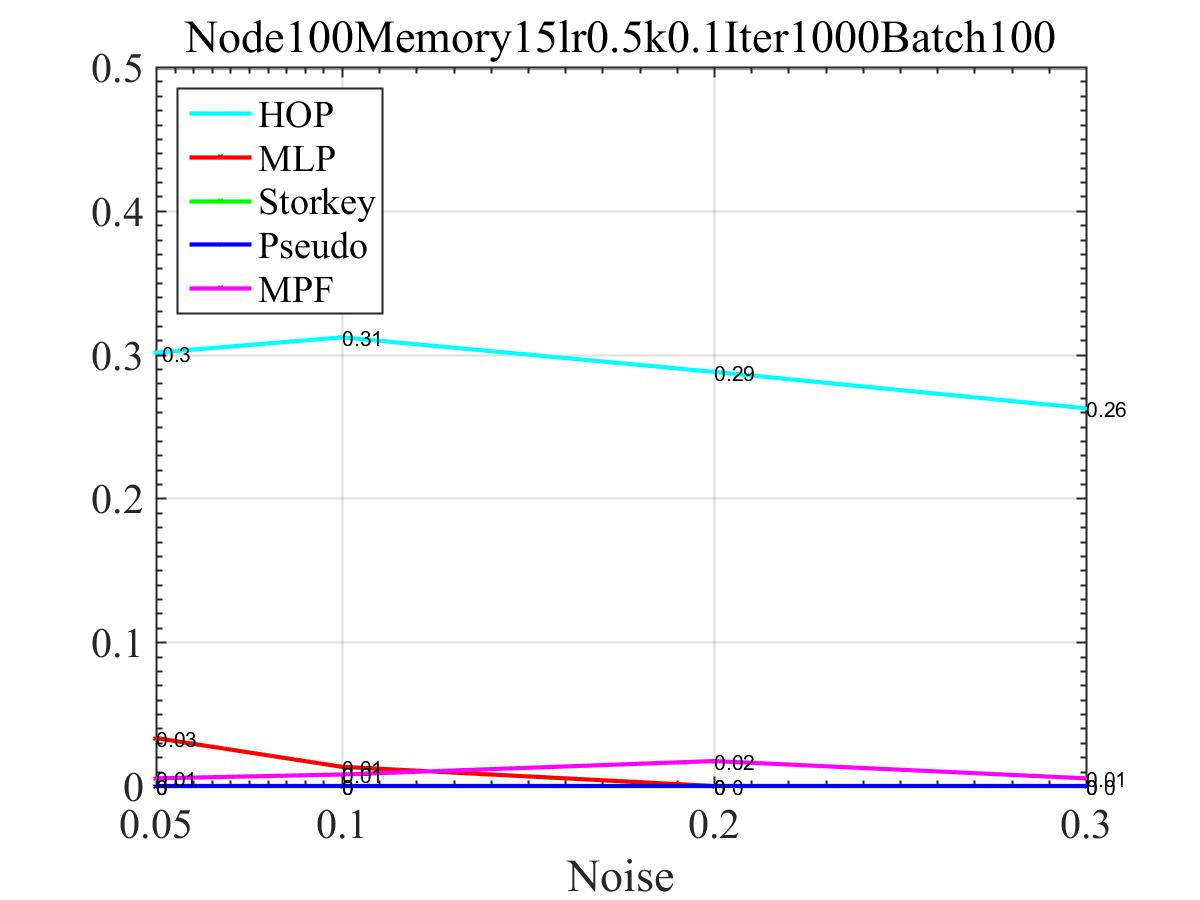
\includegraphics[width=2.2in]{Memory15Ins.jpg}
%  \caption{Memory15Ins}\label{fig:side:2c}
%\end{figure}

Third in 20 memory messages. Since the number of memory messages exceeds the capacity of Hopfield original network too more. In figure \ref{fig:fig3}, in all noise level, the error is about 12 memory messages of 20 memory messages. This also accords with the theory of capacity of Hopfield network which the capacity is 0.14$N$. And on noise level 0.05, the MLP method have 0.06 error rate. Besides on noise level 0.1, the MLP method have 0.03 error rate. This causes that MER also have 0.03 error rate.  But MPF, PSE, STO and our method MLP are almost stable on memory messages. So in figure \ref{fig:fig3} and \ref{fig:fig3}, on noise level 0.05, 0.1, and 0.2, the error rate is almost the same in all methods except HOP on metric MER and BER. The superiority of our method MLP is on noise level 0.3, both on metric MER and BER, our method MLP superior to MPF, then PSE, then STO, last is HOP.

\begin{figure*}[!h]
  \subfigure[MER]{
  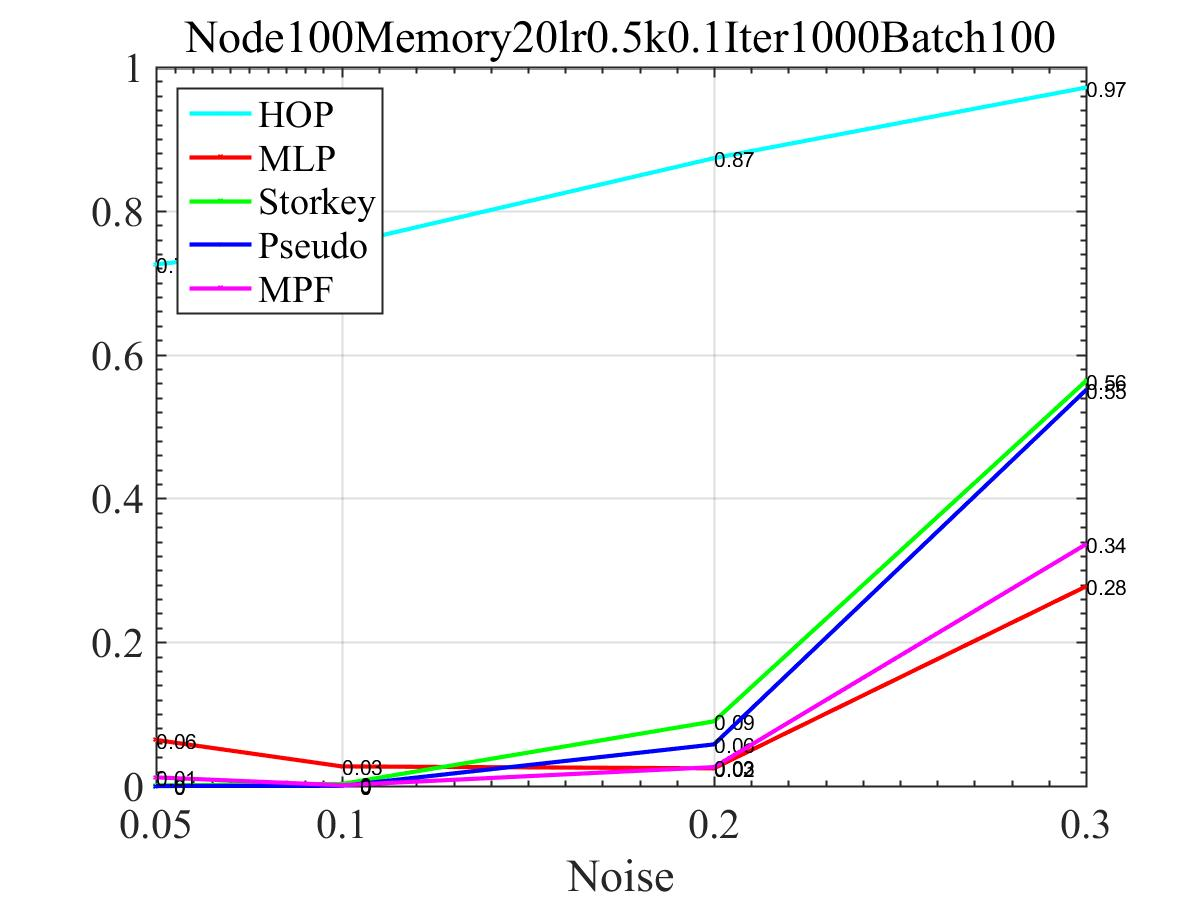
\includegraphics[width=0.35\textwidth]{Memory20MER.jpg}}
  \subfigure[BER]{
  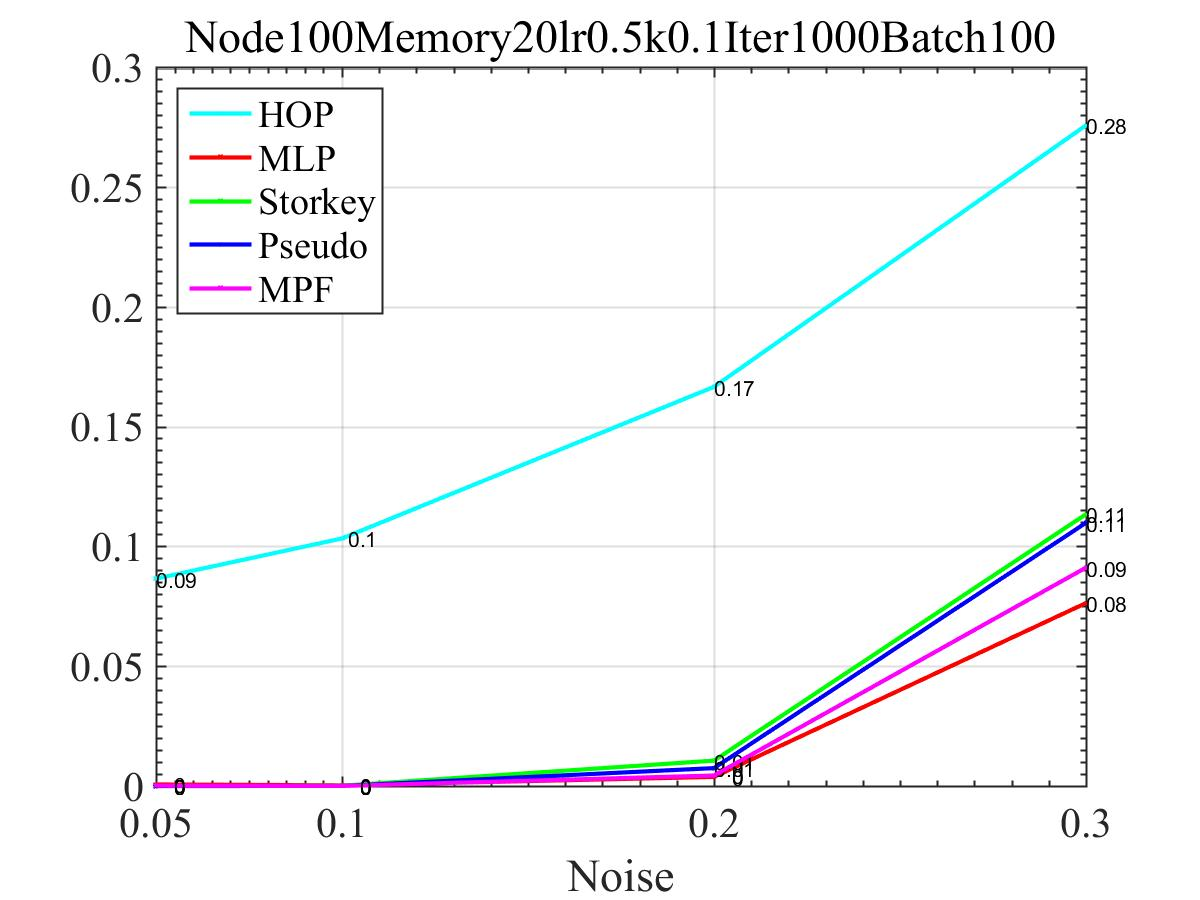
\includegraphics[width=0.35\textwidth]{Memory20BER.jpg}}
  \subfigure[Ins]{
  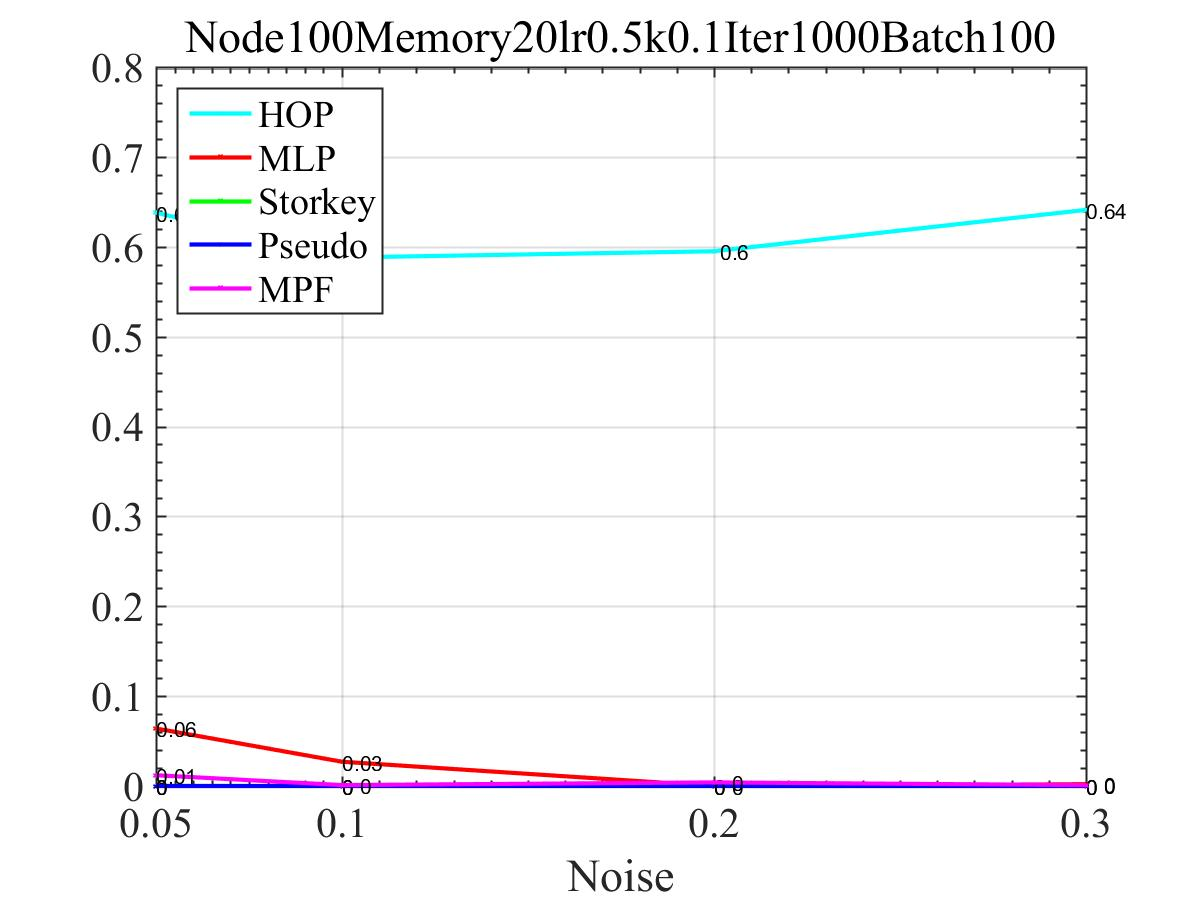
\includegraphics[width=0.35\textwidth]{Memory20Ins.jpg}}
  \caption{Memory20}
  \label{fig:fig3}
\end{figure*}

%\begin{figure}
%  \centering
%  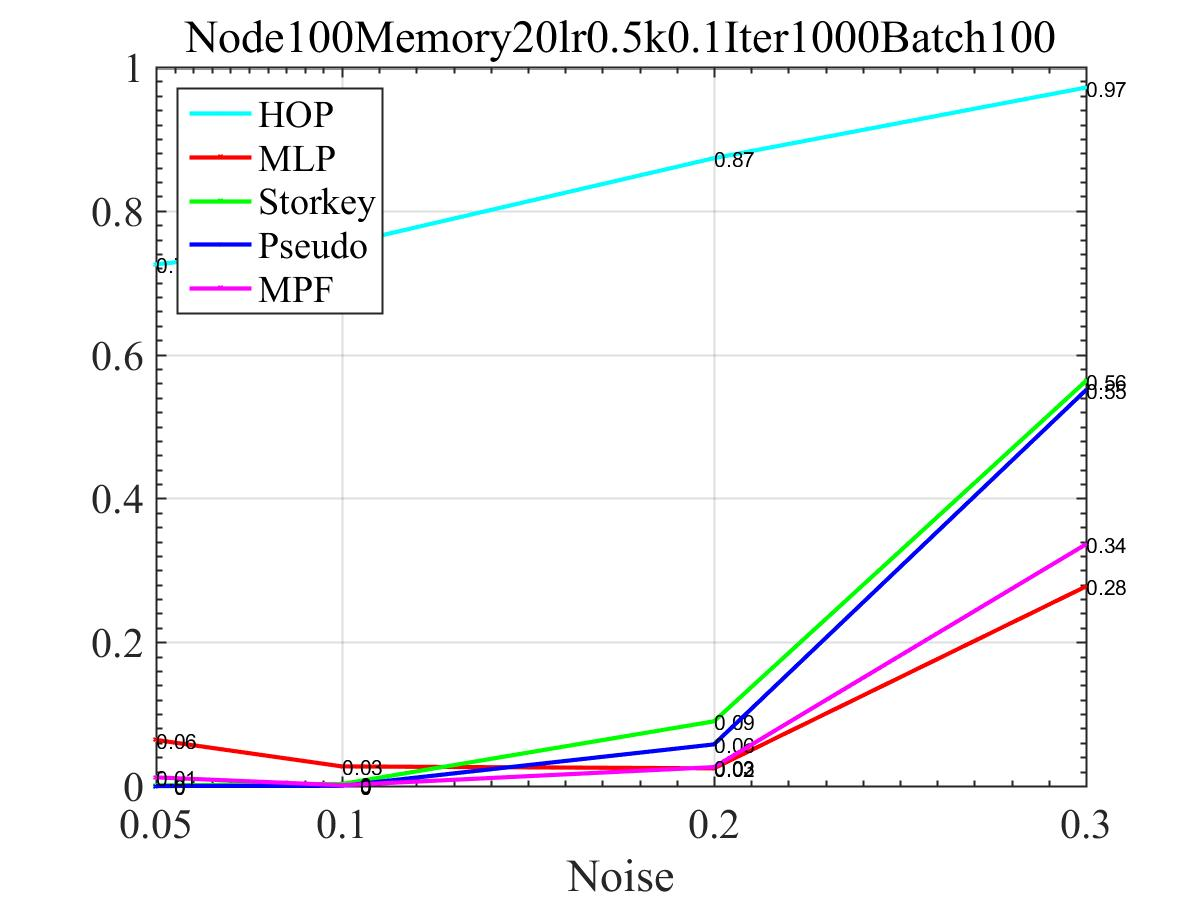
\includegraphics[width=2.2in]{Memory20MER.jpg}
%  \caption{Memory20MER}\label{fig:side:3a}
%\end{figure}
%\begin{figure}
%  \centering
%  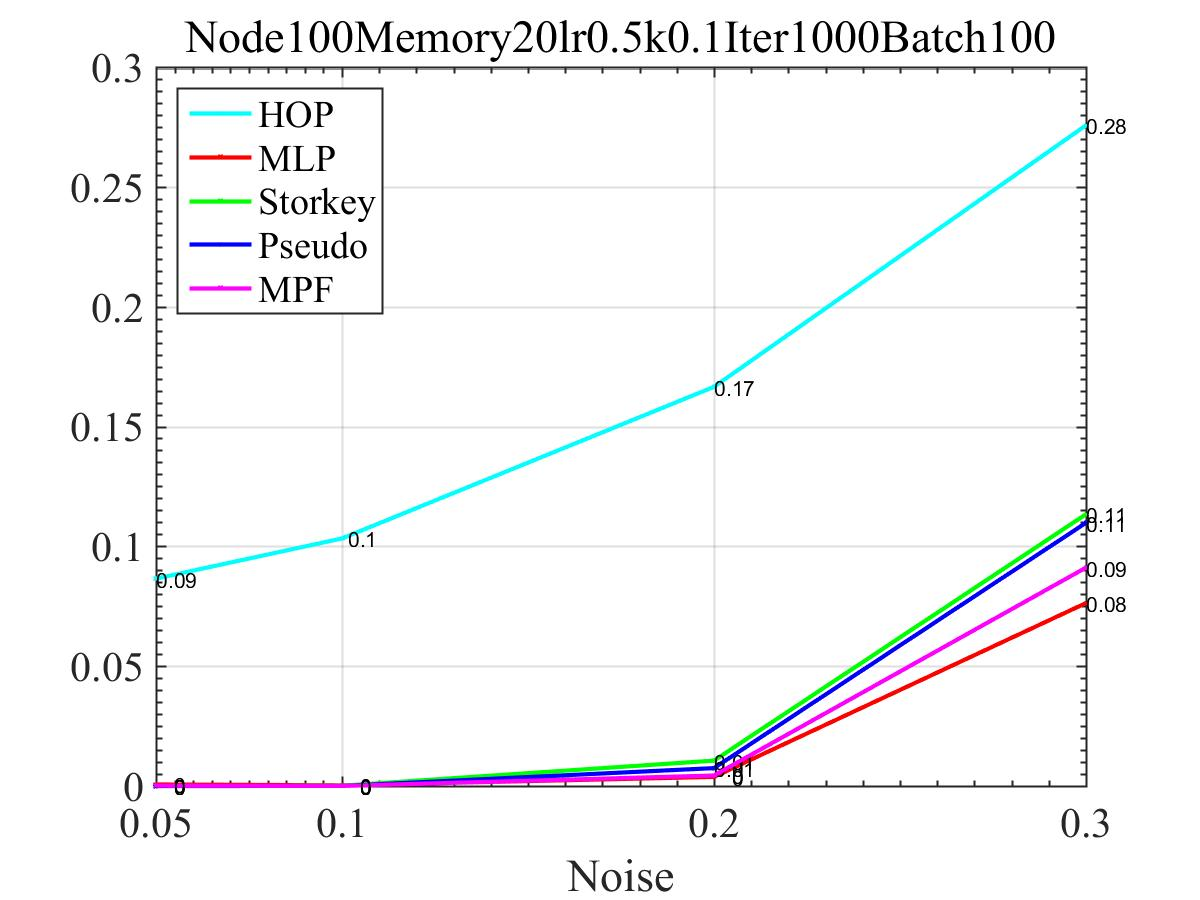
\includegraphics[width=0.48\textwidth]{Memory20BER.jpg}
%  \caption{Memory20BER}\label{fig:side:3b}
%\end{figure}
%\begin{figure}
%  \centering
%  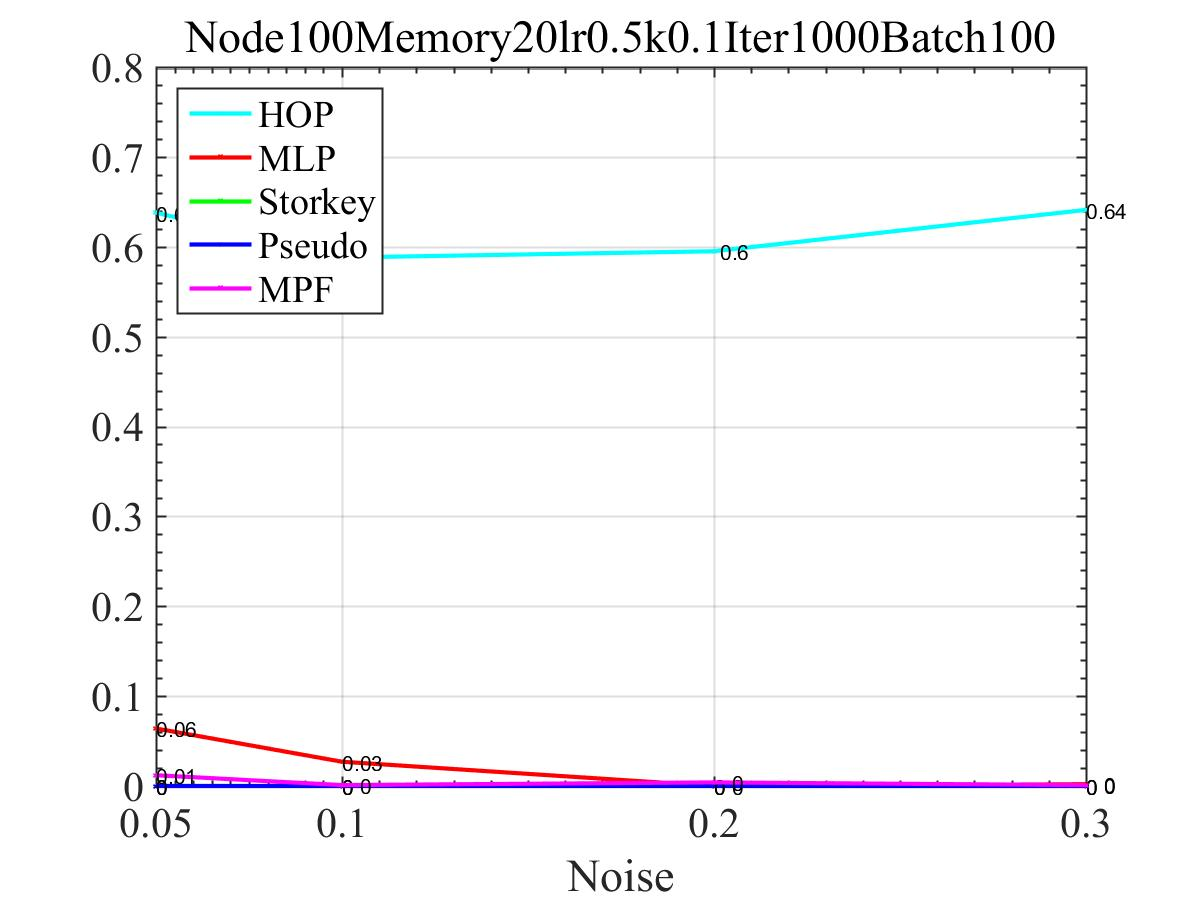
\includegraphics[width=0.48\textwidth]{Memory20Ins.jpg}
%  \caption{Memory20Ins}\label{fig:side:3c}
%\end{figure}

In summary, the weight comes from our method MLP, can make Hopfield network recover better, particularly on high noise level. When we train our Hopfield network on low noise level, maybe we cannot get the exact solution. So we try another experiment, we just train on high noise level, i.e 0.3, we test the Hopfield network on 0.1, 0.2, and 0.3. The following is the results.

\subsubsection{Experiments II} 

In these experiment II, we train our Hopfield network on high noise level, i.e 0.3 noise level. Then we do testing work on all the noise level 0.1, 0.2 and 0.3. The following figure is the results.

When there are 10 memory messages, we find that our method MLP is superior to HOP in all metric, MER, BER and Ins.
%\begin{figure}
%  \centering
%  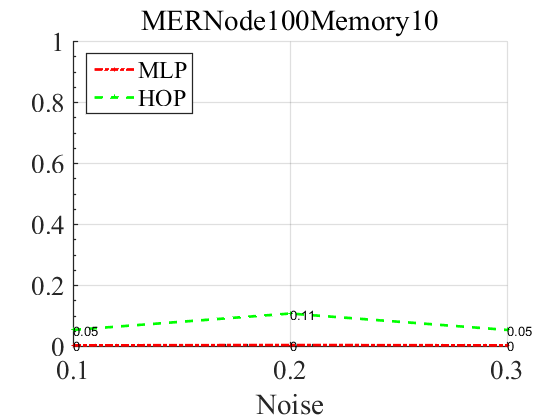
\includegraphics[width=0.48\textwidth]{E2Node100Memory10MER.png}
%  \caption{Memory10MER}\label{fig:side:4a}
%\end{figure}
%\begin{figure}
%  \centering
%  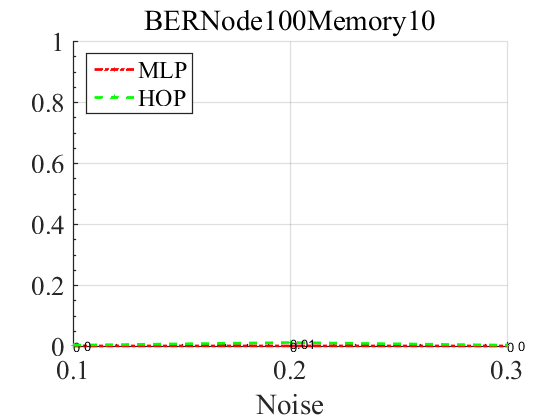
\includegraphics[width=0.48\textwidth]{E2Node100Memory10BER.png}
%  \caption{Memory10BER}\label{fig:side:4b}
%\end{figure}
%\begin{figure}
%  \centering
%  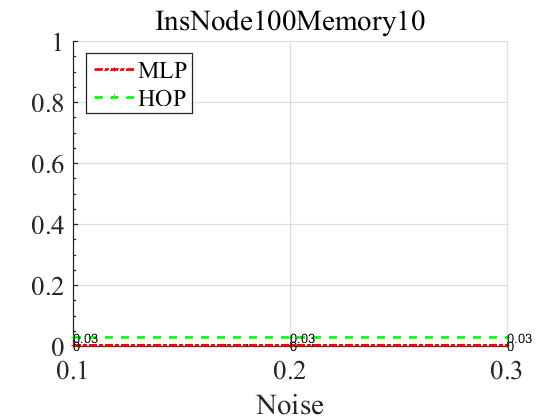
\includegraphics[width=0.48\textwidth]{E2Node100Memory10Ins.png}
%  \caption{Memory10Ins}\label{fig:side:4c}
%\end{figure}

When there are 15 memory messages, we find that our method MLP is superior to HOP in all metric, MER, BER and Ins.

%\begin{figure}
%  \centering
%  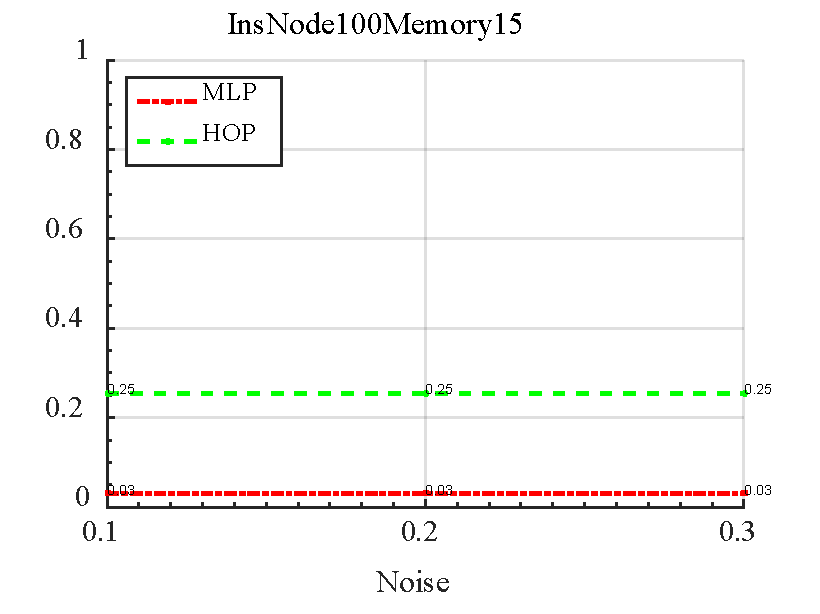
\includegraphics[width=0.48\textwidth]{Memory15Ins.pdf}
%  \caption{Memory15MER}\label{fig:side:5a}
%\end{figure}
%\begin{figure}
%  \centering
%  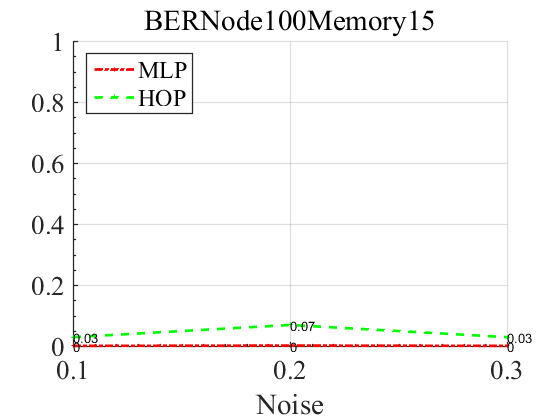
\includegraphics[width=0.48\textwidth]{E2Node100Memory15BER.png}
%  \caption{Memory15BER}\label{fig:side:5b}
%\end{figure}
%\begin{figure}
%  \centering
%  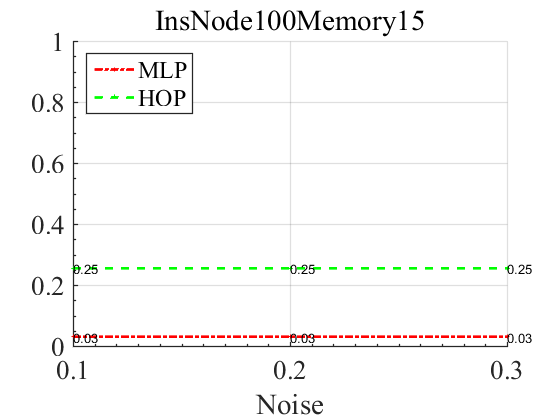
\includegraphics[width=0.48\textwidth]{E2Node100Memory15Ins.png}
%  \caption{Memory15Ins}\label{fig:side:5c}
%\end{figure}

When there are 20 memory messages, we find that our method MLP is superior to HOP in all metric, MER, BER and Ins.

%\begin{figure}
%  \centering
%  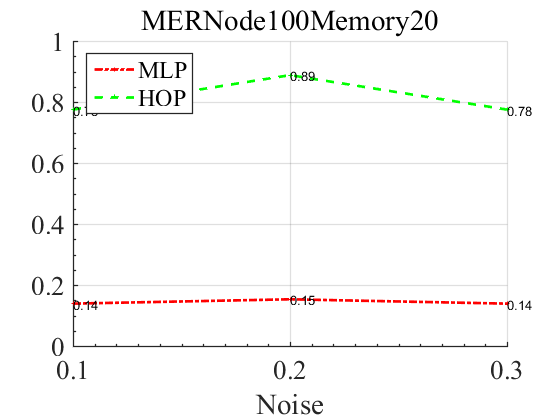
\includegraphics[width=0.48\textwidth]{E2Node100Memory20MER.png}
%  \caption{Memory20MER}\label{fig:side:6a}
%\end{figure}
%\begin{figure}
%  \centering
%  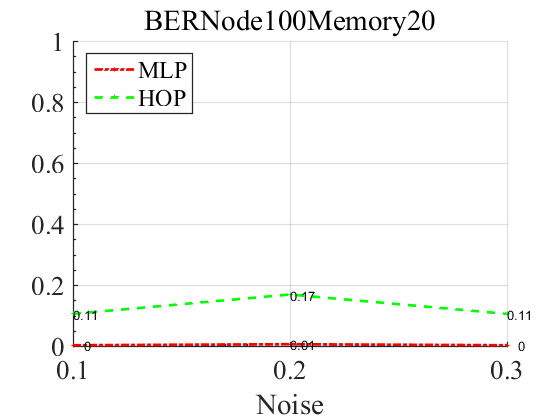
\includegraphics[width=0.48\textwidth]{E2Node100Memory20BER.png}
%  \caption{Memory20BER}\label{fig:side:6b}
%\end{figure}
%\begin{figure}
%  \centering
%  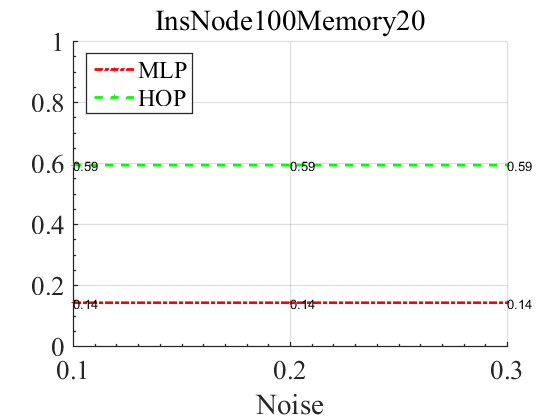
\includegraphics[width=0.48\textwidth]{E2Node100Memory20Ins.png}
%  \caption{Memory20Ins}\label{fig:side:6c}
%\end{figure}

In summary, in all three condition, our method MLP is superior to HOP 

\bibliographystyle{aaai}
\bibliography{reference}

\end{document}
